% === Begin Label Data ===
% ID: 298
% 难度星级: 4
% 标签: 数学建模
% 备注: 
% 组卷引用次数: 0
% === End  Label Data ===

\begin{problem}{1999}{G}{全国卷（理）}{22}{不等式，数列}
如图为一台冷轧机的示意图. 冷轧机由若干对轧辊组成，带钢从一端输入，经过各对轧辊逐步减薄后输出.

（1）输入带钢的厚度为 $\alpha$，输出带钢的厚度为 $\beta$，若每对轧辊的减薄率不超过 $r_0$.问冷轧机至少需要安装多少对轧辊？

（一对轧辊减薄率 $= \dfrac{\text{输入该对的带钢厚度} - \text{从该对输出的带钢厚度}}{\text{输入该对的带钢厚度}}$）

（2）已知一台冷轧机共有 $4$ 对减薄率为 $20\%$ 的轧辊，所有轧辊周长均为 $1600$. 若第 $k$ 对轧辊有缺陷，每滚动一周在带钢上压出一个疵点，在冷轧机输出的带钢上，疵点的间距为 $L_k$. 为了便于检修，请计算 $L_1$、$L_2$、$L_3$ 并填入下表（轧钢过程中，带钢宽度不变，且不考虑损耗）。

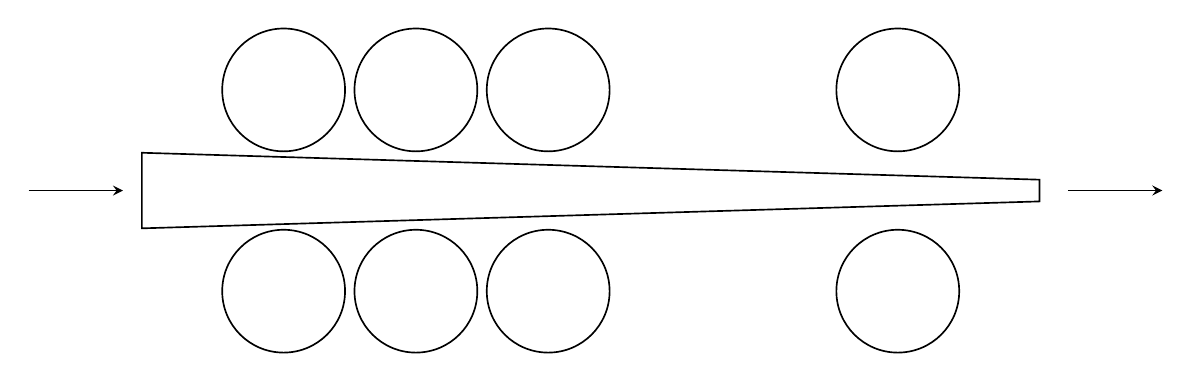
\begin{tikzpicture}[scale=1.2, >=stealth]
    % 1. 绘制中间的带钢 (从左向右逐渐变薄)
    % 左端点 x=0，右端点 x=9.5
    % 经过精确计算斜率，使其刚好与下方的轧辊相切
    \draw[semithick] (0, 0.4) -- (9.5, 0.115) -- (9.5, -0.115) -- (0, -0.4) -- cycle;

    % 2. 绘制上排轧辊 (4个圆)
    % fill=white 能够遮盖掉圆内部的带钢线条，完美还原原图效果
    \draw[semithick, fill=white] (1.5, 1.065) circle (0.65);
    \draw[semithick, fill=white] (2.9, 1.065) circle (0.65);
    \draw[semithick, fill=white] (4.3, 1.065) circle (0.65);
    \draw[semithick, fill=white] (8.0, 1.065) circle (0.65);

    % 3. 绘制下排轧辊 (4个圆，纵坐标与上排对称)
    \draw[semithick, fill=white] (1.5, -1.065) circle (0.65);
    \draw[semithick, fill=white] (2.9, -1.065) circle (0.65);
    \draw[semithick, fill=white] (4.3, -1.065) circle (0.65);
    \draw[semithick, fill=white] (8.0, -1.065) circle (0.65);

    % 4. 绘制输入与输出的指示箭头
    \draw[->, semithick] (-1.2, 0) -- (-0.2, 0);
    \draw[->, semithick] (9.8, 0) -- (10.8, 0);

\end{tikzpicture}

\begin{center}
\begin{tabular}{|c|c|c|c|c|}
\hline
轧辊序号 & 1 & 2 & 3 & 4 \\
\hline
疵点间距 $L_k$ / mm & & & & 1600 \\
\hline
\end{tabular}
\end{center}
\end{problem}

\begin{answer}
（1）$\left\lceil \log_{1-r_0} \dfrac{\beta}{\alpha} \right\rceil$；（2）$L_1 = 3125$，$L_2 = 2500$，$L_3 = 2000$.
\end{answer}

\begin{solutions}
（1）设输入带钢的初始厚度为 $h_0$，经过第 $i$ 对轧辊后的厚度为 $h_i$，其中 $i = 1, 2, \cdots, n$.

由题意知 $h_0 = \alpha$，第 $i$ 对轧辊的减薄率可以表示为 $\dfrac{h_{i-1} - h_i}{h_{i-1}}$，因为已知每对轧辊的减薄率不超过 $r_0$，所以有 $\dfrac{h_{i-1} - h_i}{h_{i-1}} \leq r_0$，由于厚度恒为正数，化简可得 $h_i \geq h_{i-1}(1 - r_0)$.

将 $i = 1, 2, \cdots, n$ 时的上述不等式依次累乘，可得经过 $n$ 对轧辊后的厚度 $h_n \geq h_0 (1 - r_0)^n$，即 $h_n \geq \alpha (1 - r_0)^n$.

要求冷轧机输出带钢的厚度为 $\beta$，为确保冷轧机的极限减薄能力足以达到该要求，须满足 $\alpha (1 - r_0)^n \leq \beta$.

不等式两边同除以 $\alpha$，整理得 $(1 - r_0)^n \leq \dfrac{\beta}{\alpha}$，因为 $0 < r_0 < 1$，所以 $0 < 1 - r_0 < 1$，对不等式两边同取以 $1 - r_0$ 为底的对数，此时不等号方向改变，得 $n \geq \log_{1 - r_0} \dfrac{\beta}{\alpha}$.

因为轧辊对数 $n$ 必须为正整数，所以至少需要安装大于或等于 $\log_{1 - r_0} \dfrac{\beta}{\alpha}$ 的最小整数对轧辊。

（2）由题意知，在轧制过程中，带钢宽度不变且不考虑损耗，故对于任意一段带钢，其体积始终保持恒定。这表明该段带钢的长度与厚度的乘积为定值。

已知每对轧辊的减薄率均为 $20\%$.

设经过第 $i$ 对轧辊后的厚度为 $d_i$，则 $d_i = d_{i-1}(1 - 20\%) = \dfrac{4}{5} d_{i-1}$，由此可知，数列 $\{d_i\}$ 是以 $\dfrac{4}{5}$ 为公比的等比数列。

当第 $k$ 对轧辊有缺陷时，其滚动一周在带钢上刚好压出两个疵点，此时这两个疵点之间包含的带钢初始长度即为该轧辊的周长 $1600$，且该段带钢此时的厚度为 $d_k$，当该段带钢继续向前传动，最终从第 $4$ 对轧辊输出时，其长度被拉伸变为最终间距 $L_k$，厚度被压缩变为 $d_4$.

根据体积守恒的等量关系，可建立等式 $1600 \times d_k = L_k \times d_4$，等式两边同除以 $d_4$，变形可得 $L_k = 1600 \times \dfrac{d_k}{d_4}$，由于数列为等比数列，所以 $\dfrac{d_k}{d_4} = \dfrac{1}{\left(\dfrac{4}{5}\right)^{4 - k}} = \left(\dfrac{5}{4}\right)^{4 - k}$.

将其代入长度等式，得 $L_k = 1600 \times \left(\dfrac{5}{4}\right)^{4 - k}$.

当 $k = 1$ 时，计算可得 $L_1 = 1600 \times \left(\dfrac{5}{4}\right)^3 = 3125$；当 $k = 2$ 时，计算可得 $L_2 = 1600 \times \left(\dfrac{5}{4}\right)^2 = 2500$；当 $k = 3$ 时，计算可得 $L_3 = 1600 \times \left(\dfrac{5}{4}\right)^1 = 2000$.

综上所述，表格中 $L_1$、$L_2$、$L_3$ 的值应分别填入 $3125$、$2500$、$2000$.
\end{solutions}